\documentclass[10pt]{article}
\usepackage{graphicx}
\usepackage[top=4cm, bottom=4cm, left=3cm, right=3cm]{geometry}

\title{Impariamo \LaTeX}
\author{4BLSA}
\date{28/04/25}


\begin{document}
\maketitle
\tableofcontents
\newpage


\section{Introduzione}
Questa è l'introduzione. 
 





\subsection{Sottosezione}
Questa è una sottosezione. Sia $\lambda$ un numero reale.
$$x+1=3$$
$$x^3$$
$$x^{3+y}$$
$$\sqrt[3]{3+x^2}$$
$$\frac{3z+4}{z^5}$$
$$\sin x$$
$$\log_{10}{\frac{1}{2}}$$
$$\epsilon_0$$
$$\lambda$$
$$\Omega$$
$$\zeta$$
$$\xi$$
$$\int_{a}^{b} f(x)dx$$
$$A\subseteq B$$
$$
L = -\frac{1}{4} G_{\mu\nu}^a G^{a\mu\nu} + \sum_{f} \bar{\psi}_f \left( i\gamma^\mu D_\mu - m_f \right) \psi_f
$$

$$
G_{\mu\nu}^a = \partial_\mu A_\nu^a - \partial_\nu A_\mu^a + g f^{abc} A_\mu^b A_\nu^c
$$

$$
D_\mu = \partial_\mu - i g A_\mu^a T^a
$$

\newpage
\section{Formule}
\subsection{Tante formule}
Scriviamo la seconda legge di Ohm:
$$R=\rho \frac{L}{A}$$
$$F=\frac{1}{4\pi\varepsilon_0}\frac{Q_1Q_2}{d^2}$$
$$\vec{F}=q\vec{E}$$
$$\Gamma=\vec{E}\cdot \Delta\vec{s}=|\vec{E}||\Delta\vec{s}|\cos\alpha$$

\begin{figure}[h!]
    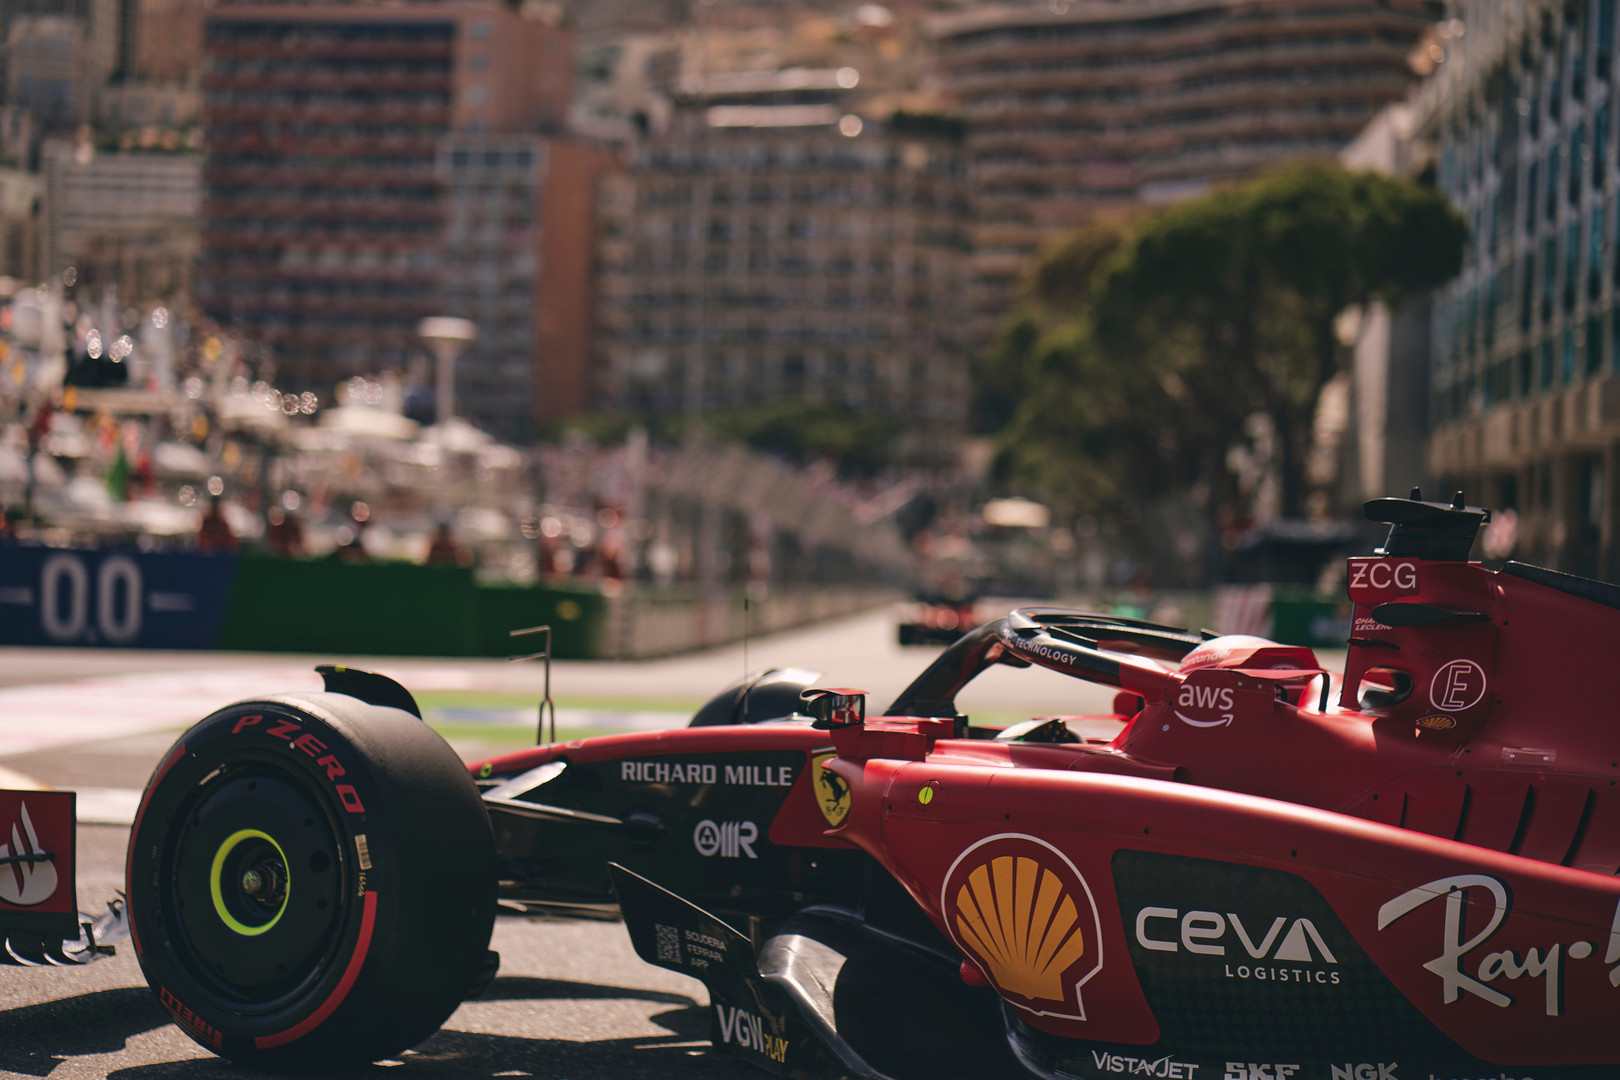
\includegraphics[width=0.5\textwidth]{pic.jpg}
    %\caption{Esempio di immagine}
\end{figure}

\begin{table}[h!]
    \centering
    \begin{tabular}{c|c|c}
        Colonna 1 & Colonna 2 & Colonna 3 \\ \hline
        Valore 1  & Valore 2  & Valore 3  \\ \hline
        Valore 4  & $F_{\mu\nu}=\partial_{\mu}A_{\nu}$  & $F=ma$  \\ 
    \end{tabular}
\end{table}

\begin{itemize}
    \item Punto 1
    \item Punto 2
    \item Punto 3
\end{itemize}

\begin{enumerate}
    \item Punto 1
    \item Punto 2
    \item Punto 3 
\end{enumerate}

\begin{equation}
    \sin x=0 \iff x=k\pi
    \label{ciao}
\end{equation}




\end{document}